% PVLDB template: bundled acmart.cls v2.19 and pvldb.sty.
\documentclass[sigconf, nonacm, pbalance]{acmart}

%%% do not modify the following VLDB block %%
%%% VLDB block start %%%
\usepackage{pvldb}
%%% VLDB block end %%%

% Publication identifiers are assigned by PVLDB only after acceptance.
\renewcommand\vldbdoi{unassigned}
\renewcommand\vldbpages{unassigned}
\renewcommand\vldbavailabilityurl{}

% Use the class's theorem styles and one shared counter within each section.
\theoremstyle{acmplain}
\newtheorem{theorem}{Theorem}[section]
\theoremstyle{acmdefinition}
\newtheorem{problem}[theorem]{Problem}
\theoremstyle{acmplain}

\newcommand{\B}{\mathcal{B}}
\newcommand{\Del}{D_{\mathrm{del}}}
\newcommand{\DeltaQ}{\Delta}
\newcommand{\MIW}{\textsc{MIW}}
\newcommand{\agg}[1]{\textnormal{\texttt{#1}}}
\DeclareMathOperator*{\argmin}{arg\,min}

\begin{document}
\title{Minimum Instability Witnesses for Aggregate Queries}
\author{Fawzi Abu Hussin}
\affiliation{%
  \institution{Ben-Gurion University of the Negev}
  \city{Beer-Sheva}
  \country{Israel}
}

\author{Yuval Moskovich}
\affiliation{%
  \institution{Ben-Gurion University of the Negev}
  \city{Beer-Sheva}
  \country{Israel}
}

\begin{abstract}
An aggregate answer can depend on a few source tuples even when its input
contains many join results. We study minimum instability witnesses:
smallest permitted deletion sets that move an aggregate answer across a
prescribed directional threshold. For positive select--project--join
queries under bag semantics, we treat COUNT, nonnegative SUM, MAX, MIN,
and AVG with immutable tuples and explicit empty-input conventions.
We relate COUNT to aggregated deletion propagation and specialize standard
submodular cover to weighted SUM with a numerical precision parameter.
For extrema, a survivor-based feasibility characterization yields a
$\min\{r,1+\ln m\}$ approximation by combining coverage greedy and
bounded-rank hitting set; $r$ bounds support size and $m$ counts critical
derivations. A fixed self-join query establishes NP-completeness of each
budget decision problem. Singleton supports are tractable for every operator, while sign separation
yields a constructive coverage subclass for AVG. We give a unified integer
linear formulation and exact marginal computation through incremental
supports, query reevaluation, and suitable arithmetic provenance circuits.
We prove when circuit derivatives equal deletion gains and explain why
AVG's signed threshold requires separate treatment. A reproducible TPC-H-derived pilot compares these execution choices for
COUNT, SUM, and AVG, validating all 180 measured witnesses against residual
SQL and exact arithmetic. The results distinguish witness-size guarantees
from representation and execution costs.
\end{abstract}

\maketitle

%%% do not modify the following VLDB block %%
%%% VLDB block start %%%
\vldbtopmatter
%%% VLDB block end %%%

\section{Introduction}
\label{sec:introduction}
Aggregate queries compress many records into a single number, but the
number of contributing records can obscure dependence on a few source
tuples. In a join, deleting one connector tuple can remove many aggregate
inputs at once. A count supported by thousands of derivations may therefore
cross a decision threshold after only a handful of source deletions.
This motivates a source-level question: how many permitted deletions are
needed to change the quantitative conclusion?

Small-deletion robustness is also studied in statistical analysis, where
removing a few observations can change an estimate or its
interpretation~\cite{broderick2020dropping,huang2025dropping}. Database
joins introduce an additional dependency: one source tuple can participate
in many output derivations. Local sensitivity measures the effect of a
single update~\cite{tao2020sensitivity}, while ranking stability studies
how changes to an item's values affect its
position~\cite{campbellLocalStability}. We instead fix an aggregate-answer
threshold and minimize the number of source deletions needed to cross it.

We call an optimal deletion set a \emph{minimum instability witness}
(\MIW). The threshold is directional: downward for \agg{COUNT},
nonnegative \agg{SUM}, and \agg{MAX}; upward for \agg{MIN}; and either
chosen direction for \agg{AVG}. Designated deletability lets an analyst
vary uncertain records while treating reference data as immutable.
Minimum cardinality is essential: an inclusion-minimal set may contain
many more deletions than necessary.

\paragraph{Relationship to deletion propagation.}
For full self-join-free conjunctive queries over duplicate-free relations,
the COUNT objective coincides with aggregated deletion propagation (ADP).
Hu et al.~\cite{hu2021adp} give logarithmic and relation-count
approximations in that shared setting. Classical view deletion and its
source/view side-effect objectives provide the broader
context~\cite{buneman2002deletion,kimelfeld2011deletion}; generalized
deletion propagation also supplies ILP methods for combined deletion and
preservation requirements~\cite{makhija2025ilp}. We build on this foundation
to explain how numerical thresholds and nonempty aggregate inputs determine
the optimization structure across five operators.

\paragraph{Three aggregate regimes.}
COUNT and nonnegative SUM yield weighted coverage: deleting a tuple removes
the nonnegative contributions of its previously surviving derivations.
MAX and MIN instead require hitting every derivation on the wrong side of
the target while preserving an acceptable survivor. Their immediate
numerical change can conceal progress until all competing extrema vanish.
AVG changes both numerator and denominator, giving a signed threshold
constraint. These regimes determine which exact and approximate methods
apply, and what the provenance representation must support.

\paragraph{Contributions.}
\begin{itemize}
\item We formalize directional \MIW\ under bag semantics with immutable
tuples and explicit empty-input conventions. We establish fixed-query
hardness for all five aggregates and exact algorithms for singleton
supports, showing that reusing a single deletable relation can move the
query class from uniform tractability to NP-complete cases
(Sections~\ref{sec:problem}--\ref{sec:complexity}).
\item We give coverage bounds for COUNT and SUM with explicit precision,
a complete extrema feasibility test, and a $\min\{r,1+\ln m\}$ extrema approximation,
where $r$ bounds support size and $m$ counts critical derivations. For AVG,
we identify a sign-separated coverage subclass alongside the general
signed formulation (Sections~\ref{sec:theory}--\ref{sec:algorithms}).
\item We specify a unified exact ILP and exact marginal computation through
incremental supports, lazy query oracles, and multilinear circuits. We
connect the derivative condition to source reuse and distinguish current
deletion gains from coalition-based attribution
(Section~\ref{sec:algorithms}).
\item We implement and compare these execution choices in a reproducible
TPC-H-derived pilot for COUNT, SUM, and AVG, validating every returned
witness by residual SQL and exact arithmetic
(Section~\ref{sec:experiments}).
\end{itemize}
Section~\ref{sec:related} situates these results in provenance, attribution,
robustness, and repair research. Section~\ref{sec:conclusion} discusses
extensions beyond the current model and evaluation.


\section{Preliminaries and Problem Formulation}
\label{sec:problem}

We study how many input tuples must be deleted to move an aggregate-query
answer across a prescribed threshold. This section specifies the query
model and defines budgeted instability witnesses. Section~\ref{sec:complexity}
studies their complexity; the subsequent coverage analysis is reserved
for Section~\ref{sec:theory}.

\subsection{Data and Query Model}
\label{sec:setting}

Let $D$ be a finite relational database instance. We identify each tuple
occurrence by a distinct identifier, so equal-valued tuples can be deleted
independently. A query $Q$ consists of a positive select--project--join
(SPJ) expression followed by a scalar aggregate. We use bag semantics:
different successful derivations contribute separately, including when
projection produces equal-valued results. We consider \agg{COUNT},
\agg{SUM}, \agg{MAX}, \agg{MIN}, and \agg{AVG}, without grouping,
negation, or duplicate elimination. For \agg{SUM}, contributions are
nonnegative. Aggregate inputs are numeric and contain no null values.

Only tuples in a designated set $\Del\subseteq D$ may be deleted; all other
tuples are immutable. A deletion set $S\subseteq\Del$ produces the instance
$D\setminus S$. Deletions can remove derivations but cannot create new ones.
There is no restriction on overlap between derivations or on which input
relations contain deletable tuples.

Let $\B$ be the multiset of successful derivations before aggregation.
For a derivation $b\in\B$, let $v_b$ be its aggregate input value and let
$T_b\subseteq\Del$ contain the deletable tuples on which it depends.
Immutable tuples are implicit in the derivation and do not appear in $T_b$.
The surviving derivations after deleting $S$ are
\begin{equation}
\label{eq:surviving-derivations}
\B(S)=\{b\in\B:S\cap T_b=\emptyset\},
\end{equation}
where multiplicities are retained. Thus, $b$ is destroyed exactly when
$S\cap T_b\ne\emptyset$. This representation follows the provenance view of query
evaluation~\cite{buneman2001whywhere,green2007provenance,amsterdamer2011aggregate}.
It describes the query semantics; it does not require an algorithm to
materialize every derivation.

We define \agg{COUNT} and \agg{SUM} on an empty input to be zero,
using the additive identity for \agg{SUM} rather than SQL's null result.
For \agg{MAX}, \agg{MIN}, and \agg{AVG}, a valid deletion set must
leave $\B(S)\ne\emptyset$. We assume that the original aggregate is defined. If a tuple is used in
multiple atom positions of a self-join derivation, it occurs only once in
$T_b$: deleting that tuple destroys the derivation once.

\paragraph{Computational input.}
For algorithmic claims, values and thresholds are binary-encoded rationals,
and the deletion budget $k$ is a binary-encoded nonnegative integer.
Data-complexity statements fix $Q$; combined complexity allows it to vary.
Write $n=|\Del|$, $M=|\B|$, and $L=\sum_{b\in\B}|T_b|$.
An explicit-derivation input lists every value and support, including bag
multiplicities. Alternatively, a database engine can evaluate residual
queries, or an explicitly specified circuit can provide value oracles.
These representations have different costs; their execution methods are
reserved for Section~\ref{sec:algorithms}.
For a fixed query with $a$ relation-atom occurrences, $M\le |D|^a$,
so enumeration is polynomial in data size, though it may be impractical.
This is not a polynomial bound in combined query/database size or in the
size of an arbitrary compressed representation. Arithmetic-operation bounds
below are distinguished from bit complexity; exact rational operations
also depend on operand lengths.

\subsection{Instability Witnesses}
\label{sec:witnesses}

Fix a deletion budget $k\in\mathbb{Z}_{\ge0}$ and a required answer
change $\theta>0$. The budget counts source tuple occurrences; the
threshold measures the change in the aggregate answer. For \agg{COUNT}, \agg{SUM},
\agg{MAX}, and \agg{AVG}, we seek a downward change and write
$\tau_{\downarrow}=Q(D)-\theta$. For \agg{MIN}, deletions cannot decrease
the minimum of a nonempty input, so we instead seek an upward change and
write $\tau_{\uparrow}=Q(D)+\theta$. Accordingly, define
\begin{equation}
\label{eq:deletion-benefit}
\DeltaQ(S)=
\begin{cases}
Q(D\setminus S)-Q(D), & \text{for \agg{MIN}},\\
Q(D)-Q(D\setminus S), & \text{otherwise}.
\end{cases}
\end{equation}
The threshold is non-strict: equality suffices to establish instability.
Unlike the other operators, \agg{AVG} can move in either direction under
deletions. We state its downward version; negating all values converts an
upward instance into a downward one with the same witnesses. A two-sided
\agg{AVG} request is solved by taking the smaller feasible witness from
the two directions, reporting infeasibility only if both fail.

\begin{definition}[$k$-instability witness]
\label{def:witness}
For a prescribed budget $k$ and threshold $\theta$, a valid deletion set
$S\subseteq\Del$ is a \emph{$k$-instability witness} if
\[
|S|\le k\qquad\text{and}\qquad\DeltaQ(S)\ge\theta.
\]
Equivalently, within the deletion budget it satisfies
$Q(D\setminus S)\le\tau_{\downarrow}$ for a downward threshold, or
$Q(D\setminus S)\ge\tau_{\uparrow}$ for \agg{MIN}.
\end{definition}

\begin{problem}[Minimum $k$-Instability Witness (\MIW)]
\label{prob:miw}
Given $D$, $Q$, $\Del$, $k\ge0$, and $\theta>0$, compute
\begin{equation}
\label{eq:miw}
\begin{aligned}
S^\star\in\argmin_{S\subseteq\Del}\{\,|S|:\;&S\text{ is valid},\\
&|S|\le k,\ \DeltaQ(S)\ge\theta\,\},
\end{aligned}
\end{equation}
or report that no witness exists within budget $k$.
\end{problem}

We require minimum cardinality, rather than merely inclusion minimality.
All deletions have unit cost. The parameters have different roles: $k$
bounds the allowed intervention, while $\theta$ fixes the required answer
change. Minimization chooses the smallest witness among those satisfying
both constraints; the budget is an upper bound, not a required size.

Let $\rho_\theta(D,Q,\Del)$ denote the minimum valid witness size without
a budget, taking value $\infty$ when no deletion set reaches the threshold.
Then a $k$-instability witness exists exactly when
\[
\rho_\theta(D,Q,\Del)\le k.
\]
When feasible, Problem~\ref{prob:miw} returns this minimum size. Failure
within a particular budget means $\rho_\theta>k$; it does not by itself
establish that the threshold is unreachable with more deletions. A larger
$\rho_\theta$ means greater directional threshold stability. In particular,
$k=0$ admits no witness because $\theta>0$.

\begin{example}
\label{ex:miw}
Consider the join $R(K)\Join V(K,A)$, with deletable tuples
$r_1=R(1)$ and $r_2=R(2)$, and immutable tuples
$V(1,4)$, $V(1,6)$, and $V(2,5)$. The sum of $A$ is $15$.
Deleting $r_1$ destroys the two derivations with values $4$ and $6$,
whereas deleting $r_2$ destroys the derivation with value $5$.
For $\theta=8$ and $k=1$, the set $\{r_1\}$ is a minimum
$1$-instability witness:
the remaining sum is $5\le15-8$, while $\{r_2\}$ does not reach the
threshold. The deletion budget concerns input tuples, not the number of
destroyed join results.
\end{example}

\paragraph{Aggregate-specific structure.}
For \agg{COUNT} and nonnegative \agg{SUM}, the numerical change in
the answer is a weighted-coverage function over destroyed derivations.
For \agg{MAX} and \agg{MIN}, the threshold instead identifies a set
of critical derivations that must all be destroyed, while at least one
other derivation survives. For \agg{AVG}, the numerical change need
not be monotone or submodular. These distinctions organize the planned
coverage and approximation analysis in Section~\ref{sec:theory}.

\paragraph{Why bag projection is essential.}
Let deletable $R(1),R(2)$ join with immutable $V(1,7),V(2,7)$ and project
$A$. Under bag semantics the result is $\{7,7\}$, and deleting either
$R$ tuple removes one copy. Duplicate elimination instead gives $\{7\}$: either deletion alone
leaves that value present, while both remove it.
The marginal \agg{COUNT} loss of the second deletion rises from zero to
one. Thus duplicate elimination can invalidate submodularity; results for
set projection cannot be imported without checking their semantics.

\section{Complexity and Tractable Cases}
\label{sec:complexity}

The \emph{budget decision problem} asks whether a $k$-instability witness
from Definition~\ref{def:witness} exists for the given $(k,\theta)$.
The optimization version additionally minimizes its size within that
budget. We first establish fixed-query hardness through source sharing,
then show that singleton supports admit exact algorithms. For the latter,
one may compute the unbudgeted optimum $\rho_\theta$ and compare it
with $k$: an optimum at most $k$ solves \MIW, while a larger optimum
certifies that no witness exists within the budget.

\begin{theorem}[Fixed-query hardness]
\label{thm:hardness}
For each of \agg{COUNT}, \agg{SUM}, \agg{MAX}, \agg{MIN}, and \agg{AVG},
the budget decision problem is NP-complete in data complexity for the
fixed body
\[
R(x)\Join E(x,y,A)\Join R(y).
\]
This holds with values in $\{0,1\}$, designated immutable tuples, and a
self-join of $R$.
\end{theorem}

\begin{figure*}[t]
\centering
\begin{tikzpicture}[
  font=\small,
  vertex/.style={circle,draw,minimum size=7mm,inner sep=0pt},
  selected/.style={vertex,fill=blue!12,draw=blue!65!black,very thick},
  support/.style={draw,rounded corners,minimum width=40mm,
                  minimum height=8mm,fill=black!2},
  flow/.style={-{Stealth[length=2.2mm]},thick,draw=black!55}]
\node[font=\small\bfseries] at (1.6,3.0) {Vertex Cover instance};
\node[vertex] (a) at (0.2,1.8) {$a$};
\node[selected] (b) at (1.6,0.9) {$b$};
\node[vertex] (c) at (3.0,1.8) {$c$};
\draw[thick] (a)--(b)--(c);
\node[align=center] at (1.6,0.05) {$k=1$, cover $C=\{b\}$};

\draw[flow] (3.6,1.5)--(4.5,1.5);
\node[font=\small\bfseries] at (7.0,3.0) {Database instance};
\node[anchor=north] at (5.5,2.5) {\begin{tabular}{c}
  $R$\\\hline
  $a$\\
  \textcolor{blue!65!black}{$\boldsymbol{b}$}\\
  $c$
\end{tabular}};
\node[anchor=north] at (7.9,2.5) {\begin{tabular}{ccc}
  \multicolumn{3}{c}{$E(x,y,A)$}\\\hline
  $a$ & $b$ & $1$\\
  $b$ & $c$ & $1$
\end{tabular}};
\node[align=center] at (7.0,0.05) {$R$ deletable; $E$ immutable};

\draw[flow] (9.4,1.5)--(10.3,1.5);
\node[font=\small\bfseries] at (12.9,3.0) {Derivation supports};
\node[support] at (12.9,2.1)
  {$T_{ab}=\{R(a),\textcolor{blue!65!black}{R(b)}\}$};
\node[support] at (12.9,1.15)
  {$T_{bc}=\{\textcolor{blue!65!black}{R(b)},R(c)\}$};
\node[align=center] at (12.9,0.05)
  {Delete $S=\{R(b)\}$; both die};

\node[draw=black!25,fill=black!3,rounded corners,minimum width=15cm,
      align=center,inner sep=6pt] at (7.55,-0.95)
  {For COUNT and SUM, $Q(D)=2$ and $\theta=2$.\\
   $C$ covers every edge $\Longleftrightarrow$ $S$ destroys every edge derivation;
   $|C|=|S|\le k$.};
\end{tikzpicture}
\caption{A budget-preserving NP-hardness reduction from Vertex Cover for COUNT and SUM,
illustrated with two edges and $k=1$. For a general graph, each vertex
becomes a deletable $R$ tuple and each oriented edge becomes one immutable
$E$ tuple. The fixed body $R(x)\Join E(x,y,A)\Join R(y)$ gives one
support per edge. Setting $\theta=|E_G|$ forces all edge supports to be
hit. The proof extends the construction to MAX, MIN, and AVG using a
permanently surviving derivation; the same budget $k$ is retained.}
\label{fig:vertex-cover}
\Description{Three panels show the reduction. In the left panel, the graph
has edges a-b and b-c, and vertex b alone covers both. The middle panel
contains deletable R tuples a, b, c and immutable E tuples (a,b,1) and
(b,c,1). The right panel shows the supports R(a),R(b) and R(b),R(c).
Deleting the single tuple R(b) destroys both derivations, preserving the
Vertex Cover budget of one.}
\end{figure*}

\begin{proof}
Reduce from Vertex Cover on a simple undirected graph $G=(V,E_G)$ with
at least one edge and Vertex Cover budget $k$. We use exactly the same
budget $k$ in the \MIW\ instance. Orient each edge once. Create a deletable tuple $R(v)$
for each vertex and an immutable tuple $E(u,v,1)$ for each oriented edge.
There is exactly one derivation per edge, with support
$\{R(u),R(v)\}$. A deletion set destroys every such derivation exactly
when its vertices form a vertex cover. Figure~\ref{fig:vertex-cover}
illustrates this correspondence.

For \agg{COUNT} and \agg{SUM}(A), choose $\theta=|E_G|$. The target
is zero. A vertex cover of size at most $k$ therefore exists if and only
if the constructed instance has a $k$-instability witness. For \agg{MAX} and
\agg{AVG}, add fresh vertices $p,q$, immutable $R(p),R(q)$, and
immutable $E(p,q,0)$. This creates one permanently surviving zero-valued
derivation and no additional joins. For \agg{MAX}, use $\theta=1$.
For \agg{AVG}, use $\theta=|E_G|/(|E_G|+1)$, the initial average.
In either case, the target is zero and is reached precisely when every
graph-edge derivation is destroyed. For \agg{MIN}, instead give all
graph edges value zero and the permanent edge value one; choose
$\theta=1$. Reaching minimum one again requires destroying every graph
edge. In every construction, feasible deletion sets and vertex covers
have the same cardinalities, so the budget $k$ is preserved for every
aggregate. The encoding has polynomial size.

For membership in NP, a certificate lists at most $k$ deletable tuples.
Evaluation of this fixed query, the aggregate, and the validity condition
uses polynomial time with exact rational arithmetic. Hence the decision
problem is NP-complete for each operator.
\end{proof}

Only $R$ contains deletable tuples in this construction. Reusing that one
relation in two atom positions is sufficient for hardness across all five
operators. Each support has size two: pairwise coupling inside a single
deletable relation is already sufficient for this reduction.

\begin{proposition}[Singleton-support coverage]
\label{prop:modular}
For \agg{COUNT} or nonnegative \agg{SUM}, suppose $|T_b|\le1$ for
every $b$. Sort deletable tuples by their initial marginal gains. The
shortest prefix reaching the threshold is a minimum $k$-instability
witness if its size is at most $k$; otherwise no witness fits the budget.
Equivalently, feasibility is decided by the total gain of the largest
$\min\{k,n\}$ gains.
\end{proposition}
\begin{proof}
Put $a_t=\sum_{b:T_b=\{t\}}w_b$. The benefit is modular:
$f(S)=\sum_{t\in S}a_t$. Among sets of any fixed cardinality $j$, the
$j$ largest $a_t$ attain the greatest possible benefit. The first feasible
prefix therefore has minimum cardinality. If that prefix exceeds $k$,
no set of at most $k$ deletions can reach the threshold.
\end{proof}
The gains can be computed in $O(M+n)$ operations from explicit singleton
supports, followed by $O(n\log n)$ comparisons for sorting.

\begin{theorem}[Singleton-support tractability]
\label{thm:single-relation}
If $|T_b|\le1$ for every derivation, \MIW\ is solvable in polynomial
time for each of the five aggregates. Consequently, every fixed
self-join-free query with only one deletable relation is tractable.
Allowing that relation to occur twice already admits the fixed-query
NP-complete cases of Theorem~\ref{thm:hardness}.
\end{theorem}
\begin{proof}
Proposition~\ref{prop:modular} handles COUNT and SUM. For an extremum,
each critical singleton forces its tuple's deletion; an empty critical
support makes the instance infeasible. The union of forced tuples is
optimal if any derivation survives, and otherwise no valid witness exists.
If the forced set exceeds $k$, the budgeted instance is infeasible.

For AVG at target $\tau=\tau_{\downarrow}$, define
$F_\tau(S)=\sum_{b\in\B(S)}(v_b-\tau)$ and write
$F_0=F_\tau(\emptyset)>0$.
Let $a_t$ sum $v_b-\tau$ over the derivations with $T_b=\{t\}$.
Singleton supports give
\[
F_\tau(S)=F_0-\sum_{t\in S}a_t.
\]
Every valid threshold-crossing witness preserves a derivation $b_0$ with
$v_{b_0}\le\tau$.
Enumerate its possible support, forbid deleting that support, sort the
remaining positive $a_t$ in descending order, and take the shortest
prefix whose sum reaches $F_0$. This is exact for that protected domain:
nonpositive gains never help, and the largest gains maximize benefit for
each cardinality. Taking the smallest feasible prefix over survivors is
therefore globally optimal before imposing the budget; compare its size
with $k$ to solve the budgeted problem. At most $n+1$ distinct singleton or empty
supports are protected. One initial sort and a scan per protected support
take $O(M+n\log n+n^2)$ operations and comparisons.
\end{proof}
This is a boundary of uniform tractability under a syntactic restriction:
all queries on the self-join-free side are tractable, while the expanded
class contains hard queries. Individual queries with self-joins can still
be tractable. The following independent-row case gives a faster AVG
algorithm when every deletable group has exactly one row.

\begin{proposition}[Independent-row averages]
\label{prop:avg-rows}
For a bag of numeric rows, with each deletable row contributing exactly
one aggregate input independently of other rows, downward \agg{AVG}
\MIW\ is solvable by sorting and scanning prefixes in $O(N+n\log n)$
arithmetic operations and comparisons, where $N$ is the total row count.
\end{proposition}
\begin{proof}
Sort deletable values as $u_1\ge\cdots\ge u_n$. Let $V$ be the initial
sum. For a fixed deletion count $j<N$, the remaining denominator is
$N-j$, so deleting the largest $j$ values minimizes the remaining
average. Check
\[
V-\sum_{i=1}^j u_i\ \le\ \tau_{\downarrow}(N-j)
\]
for each $j\le\min\{k,n\}$ with $j<N$, and return the first feasible
prefix. If none succeeds, no witness exists within budget $k$. One pass computes the
initial sum and prefix sums after sorting. The restriction $j<N$
ensures nonemptiness, including when every row is deletable.
\end{proof}
This case has no joins or shared supports. It illustrates why the failure
of AVG submodularity alone is not a hardness proof.

\section{Coverage and Approximation}
\label{sec:theory}
\label{sec:aggregate-submodularity}

\section{Exact Formulations and Greedy Execution}
\label{sec:algorithms}

We separate three questions: how a deletion set is represented, how its
benefit is computed, and which optimization rule chooses the next tuple.
A compact representation does not by itself provide cheap marginal gains,
and an approximate marginal oracle need not preserve an exact-greedy
guarantee.

\subsection{A Unified Explicit-Derivation ILP}
\label{sec:ilp}

Introduce binary variables $x_t$ for $t\in\Del$, with $x_t=1$ denoting
deletion, and $z_b$ for $b\in\B$, with $z_b=1$ denoting survival.
Minimize
\begin{equation}
\label{eq:ilp-objective}
\sum_{t\in\Del}x_t
\end{equation}
subject to the linking constraints
\begin{align}
 z_b&\le 1-x_t &&(b\in\B,\ t\in T_b),\label{eq:ilp-upper}\\
 z_b&\ge 1-\sum_{t\in T_b}x_t &&(b\in\B).\label{eq:ilp-lower}
\end{align}
For \agg{COUNT} or \agg{SUM}, add
\begin{equation}
\label{eq:ilp-coverage}
\sum_{b\in\B}w_b(1-z_b)\ge\theta,
\end{equation}
where $w_b=1$ or $v_b$, respectively. For \agg{MAX} or \agg{MIN}, add
\begin{equation}
\label{eq:ilp-extrema}
z_b=0\quad(b\in\B_{\mathrm{crit}}),
\qquad \sum_{b\in\B}z_b\ge1.
\end{equation}
For downward \agg{AVG}, add
\begin{equation}
\label{eq:ilp-avg}
\sum_{b\in\B}(v_b-\tau_{\downarrow})z_b\le0,
\qquad \sum_{b\in\B}z_b\ge1.
\end{equation}
Binary rational coefficients may be cleared by positive denominators
without changing feasibility.

\begin{theorem}[Exactness of the ILP]
\label{thm:ilp}
The feasible ILP solutions correspond exactly to valid instability
witnesses through $S=\{t:x_t=1\}$. Its optimum is $|S^\star|$;
ILP infeasibility is equivalent to witness infeasibility.
\end{theorem}
\begin{proof}
If any $t\in T_b$ is deleted, constraint~\eqref{eq:ilp-upper} forces
$z_b=0$. If none is deleted, constraint~\eqref{eq:ilp-lower} forces
$z_b=1$. In particular, an empty support forces survival. Thus $z_b$
is precisely the actual survival indicator. Constraint~\eqref{eq:ilp-coverage}
then expresses the destroyed contribution. Lemma~\ref{lem:extrema-equivalence}
proves the extrema constraints, and multiplying the average inequality
by its positive denominator proves~\eqref{eq:ilp-avg}. Conversely,
assigning the true deletion and survival indicators of any valid witness
satisfies every constraint for its operator. The objective counts exactly
the deleted source tuples.
\end{proof}

Both linking directions matter. With values $\{10,0\}$, only the
high-valued row deletable, and target zero, the upper bounds alone would
allow setting both $x_{10}=0$ and $z_{10}=0$, inventing a free deletion.
The lower bound prevents this spurious solution.

The encoding has $n+M$ binary variables and $O(M+L)$ constraints.
It is polynomial in the explicit-derivation representation, not necessarily
in a supplied compact circuit. It provides an exact baseline when solved
to proven optimality. A timed-out feasible solution is an upper bound on
optimum; a solver's certified lower bound is needed to quantify its gap.
The use of deletion and witness variables follows established deletion
propagation ILP methodology~\cite{makhija2025ilp}; we do not claim the
existence of such an encoding as a new optimization technique, or transfer
integral-relaxation results to this formulation without proof.

\subsection{Explicit Supports and Incremental Coverage}
\label{sec:explicit-greedy}

For nonnegative coverage weights, store an incidence list of derivations
containing each tuple and a live flag for every derivation. Initialize
\[
g_t=\sum_{b:t\in T_b}w_b.
\]
At each iteration, choose an allowed undeleted tuple of maximum $g_t$.
For each still-live derivation containing it, mark that derivation dead
and subtract $w_b$ from the gain of every tuple in its support. Dead
derivations are never subtracted again. Maintain the accumulated destroyed
weight to test termination. For extrema, use only critical derivations,
unit weights, and the permitted ground set of the current protected run.

\begin{proposition}[Incremental marginal invariant]
\label{prop:incremental}
After any deletion set $S$ selected by this procedure, every remaining
allowed tuple satisfies $g_t=f(t\mid S)$. The procedure therefore
implements exact marginal-gain greedy.
\end{proposition}
\begin{proof}
Initially every derivation is live, so the formula is
Equation~\eqref{eq:coverage-marginal}. When a tuple is deleted, precisely
the previously live incident derivations cease to survive. Their weights
are removed once from every remaining tuple's gain, leaving exactly the
sum over still-surviving incident derivations.
\end{proof}

With a scan to select the next tuple, one run takes $O(M+L+n^2)$
arithmetic operations: the incidence lists are initialized once, each
derivation dies at most once, and its support is traversed once when it
dies. Scanning the chosen tuples' incidence lists costs at most $L$ over
the run. Space is $O(M+L+n)$. These costs exclude construction of the
derivation representation. The bound is for one protected run; gains and
live flags must be reinitialized for another survivor.

The disjoint-support method can be implemented by scanning reduced critical
supports while maintaining their selected union. Add a support exactly
when its intersection with that union is empty. One protected run takes
$O(M+L+n)$ time and space with indexed tuple membership. Hence the
bounded-support guarantee does not require solving an optimization
subproblem beyond the survivor enumeration.

\subsection{Query Oracles and Exact Lazy Selection}
\label{sec:query-oracles}

Let $C_Q$ bound an exact evaluation of the residual aggregate, including
arithmetic on its encoded values. For \agg{COUNT} and \agg{SUM},
\[
f(t\mid S)=Q(D\setminus S)-Q(D\setminus(S\cup\{t\})).
\]
Caching the current answer lets ordinary greedy compute all candidates by
at most $n$ residual evaluations per iteration. At most $n$ iterations
therefore require $O(n^2)$ evaluations and $O(n^2 C_Q)$ time. For extrema,
counting residual derivations satisfying the strict critical-value test
gives the corresponding $h$ oracle under bag semantics. Survivor enumeration
still requires a complete method of obtaining safe supports; value-oracle
access alone does not supply them.

Submodularity also permits the standard accelerated greedy
selection~\cite{minoux1978lazy}. Store a previously
computed marginal as an upper bound in a max-priority queue. Recompute
the largest bound at the current deletion set. Select its tuple only when
its exact gain is at least every other stored bound; otherwise update the
bound and continue. Since true gains can only decrease, that acceptance
condition certifies an actual maximum marginal. Fixing a common tuple
order resolves ties consistently with ordinary greedy. Refreshing each
tuple at most once per iteration gives the same $O(n^2)$ worst-case oracle
bound, with additional queue overhead; fewer evaluations are a possible
practical benefit, not a worst-case improvement established here.

Restricting candidates to an uncertified active set, using estimated gains,
or accepting a tuple before this maximum test defines a heuristic. Such
choices need a separate analysis and do not inherit
Theorem~\ref{thm:general-greedy} from the implementation alone.

\subsection{Arithmetic Provenance Circuits}
\label{sec:circuits}

A circuit oracle here is an acyclic arithmetic circuit with rational
constants, tuple-survival inputs $y_t$, and binary addition and
multiplication gates. Its size $c$ counts gates and wires. The oracle
contract is that, at every Boolean assignment, its output equals the
surviving weighted derivation sum:
\begin{equation}
\label{eq:circuit-contract}
P(y)=\sum_{b\in\B}w_b\prod_{t\in T_b}y_t
\qquad(y\in\{0,1\}^{n}).
\end{equation}
Here $y_t=0$ denotes deletion. The contract may be instantiated for SUM,
COUNT, or critical COUNT. Constructing a compact circuit satisfying it
is a separate task; an arbitrary circuit for query existence is
insufficient. This arithmetic representation is motivated by semiring
provenance~\cite{green2007provenance}.

A topological evaluation takes $O(c)$ arithmetic operations. At the
assignment $y^S$ encoding the current deletions, exact marginal gains are
\begin{equation}
\label{eq:circuit-difference}
f(t\mid S)=P(y^S)-P(y^S\text{ with }y_t=0).
\end{equation}
Thus any circuit meeting the Boolean contract implements exact greedy
in $O(n^2c)$ arithmetic operations per run, without expanding its
polynomial. Protected runs fix the survivor's inputs to one and exclude
them from deletion candidates. Arithmetic complexity excludes circuit
construction and must be augmented by operand bit lengths. The contract
alone does not bound those lengths for arbitrary supplied circuits.

\begin{proposition}[Exact derivatives for multilinear circuits]
\label{prop:gradient}
If the circuit's formal polynomial is multilinear in every deletable
variable, all current deletion marginals can be computed by one forward
and one reverse differentiation pass, using $O(c+n)$ arithmetic operations.
One greedy run then uses $O(n(c+n))$ such operations, including selection.
\end{proposition}
\begin{proof}
For any undeleted tuple $t$, multilinearity gives
$P(y)=y_t A(y_{-t})+B(y_{-t})$. The difference between setting $y_t$ to
one and to zero is $A(y_{-t})=\partial P/\partial y_t$. A forward pass
records gate values. The reverse pass uses standard arithmetic-circuit
differentiation~\cite{baur1983derivatives}. In reverse topological order, initialize the output's
adjoint to one; an addition gate passes its adjoint to both inputs, and a
product gate passes its adjoint times the other input's value. Sum
adjoints at shared gates and at all leaves with the same tuple label.
The chain rule gives all partial derivatives in one pass over gates and
wires, with no division and hence no difficulty at zero-valued inputs.
Scanning the at most $n$ candidates chooses an exact largest gain.
Repeating for at most $n$ iterations gives the stated cost.
\end{proof}

Formal multilinearity is stronger than Boolean agreement with
Equation~\eqref{eq:circuit-contract}. A provenance polynomial for a
self-join may contain $y_t^2$: its values at zero and one represent one
surviving derivation, but its derivative at one is two, whereas the
actual deletion loss is one. Ordinary differentiation therefore need
not compute exact gains for self-joins. Direct reevaluation via
Equation~\eqref{eq:circuit-difference} remains correct.

The usual derivation polynomial of a self-join-free query is multilinear
in tuple identifiers. A sufficient circuit-level certificate is that, at
every multiplication gate, the two child polynomials use disjoint sets of
deletable variables. Addition can share variables between its children.
This certificate can be checked by propagating variable sets through the
DAG, with a cost depending on their representation. We do not assume
that every factorized provenance representation has this property, nor
that converting one to a multilinear circuit preserves size.

\subsection{AVG Search and Verification}
\label{sec:avg-search}

At target $\tau=\tau_{\downarrow}$ define
\[
F_\tau(S)=\sum_{b\in\B(S)}(v_b-\tau).
\]
A valid AVG witness satisfies $F_\tau(S)\le0$ and $|\B(S)|\ge1$.
A natural heuristic chooses a tuple maximizing the net decrease
$F_\tau(S)-F_\tau(S\cup\{t\})$ among deletions leaving a survivor.
The gain must include all destroyed derivations, including those with
negative $v_b-\tau$; summing only positive coefficients is not the true
threshold gain. Signed weights invalidate the monotone-coverage argument.
A run may stall without proving infeasibility, so the ILP is the exact
fallback when a certificate is required. Independent-row instances instead
use Proposition~\ref{prop:avg-rows}.

Every returned candidate should be checked against the original residual
query with the prescribed bag semantics, deletability policy, and empty-input
condition. This check certifies feasibility, not optimality. In particular,
removing redundant deletions can yield an inclusion-minimal witness without
establishing minimum cardinality. Applying that postprocessing to a feasible
approximation can only improve its size, provided each removal preserves
validity and the threshold.

\section{Experimental Evaluation}
\label{sec:experiments}

We evaluate the execution choices of Section~\ref{sec:algorithms} in a
bounded, reproducible pilot. The questions are whether the exact-greedy
implementations agree, how their setup and search costs compare with the
full ILP, and how signed-threshold greedy behaves for AVG. The experiment
uses TPC-H data~\cite{tpch} with a derived scalar query, rather than the
standard TPC-H query suite or its throughput metric.

\subsection{Workload and Measurement Protocol}

The query joins Customer, Orders, Lineitem, and Part on their standard
foreign keys and selects line items shipped in January 1995. Only Customer
and Part tuples are deletable; Orders and Lineitem are immutable. Each
surviving join derivation contributes one COUNT input or its extended price
for SUM and AVG. Prices are represented in integer cents. The two existing
TPC-H databases have scale factors 0.01 and 0.03, yielding respectively
714 and 2,358 derivations, and 949 and 3,128 contributing deletable tuples.
All supports have rank two. We use downward changes of 10\%, 25\%, and
50\% of the initial COUNT/SUM answer, rounding the required loss upward
to an integer. For AVG we use exact rational targets 2\%, 5\%, and 10\%
below its initial value.

The COUNT/SUM methods are: (i) the full survival-variable ILP of
Section~\ref{sec:ilp}; (ii) incremental-support greedy with a scan for the
largest gain; (iii) certified lazy greedy whose marginal queries run in
SQL on a materialized derivation table; and (iv) a circuit pass computing
the exact derivatives of
\[
P(y)=\sum_c y_c\sum_{b:\,c_b=c}w_b y_{p_b}.
\]
This last method specializes the multilinear oracle to the workload's
Customer/Part supports. It evaluates the inner sums and their derivatives
directly; circuit compilation and compression are separate questions.
AVG compares the full ILP with the net signed-gain heuristic of
Section~\ref{sec:avg-search}.

The machine uses an Apple M5, macOS, and Python 3.9.6. Methods run
sequentially with DuckDB 1.4.3~\cite{duckdb2019}, PuLP 3.3.0, and
HiGHS 1.12.0~\cite{highs}.
DuckDB and HiGHS use one thread. Each ILP has a five-second solve limit
and zero requested MIP gaps. Each combination of scale, aggregate, and threshold is repeated
three times, with algorithm order shuffled using seed 1729.
These are timing repetitions on fixed inputs. The 18 cases yield 180
method runs, including 54 ILP runs. Method time includes initialization,
model construction or SQL materialization, and optimization. Shared
source extraction and independent verification are excluded; extraction
took 6.3--6.9\,ms per database. We report medians and min/max timing ranges.

For every returned set, we recompute both the surviving derivation bag and
the residual SQL aggregate on the original database. Integer/rational
checks enforce the threshold and, for AVG, nonemptiness. We also require
identical selection traces for the three exact-greedy implementations.
The records retain each witness, solver status and bound, repetition,
input digest, and environment information. The accompanying experiment
artifacts include an analysis script that audits these records and
regenerates the table and figure.

% Generated by experiments/summarize_review.py from frozen measurements.
\begin{table}[t]
\centering
\caption{Optimal witness sizes in the TPC-H-derived pilot. Every measured greedy variant attained these sizes; each case has three timing repetitions.}
\label{tab:pilot-sizes}
\small
\begin{tabular}{@{}lrrr@{}}
\toprule
Aggregate & Decrease (\%) & SF 0.01 & SF 0.03\\
\midrule
\agg{COUNT} & 10 & 14 & 39\\
\agg{COUNT} & 25 & 40 & 121\\
\agg{COUNT} & 50 & 95 & 311\\
\agg{SUM} & 10 & 11 & 34\\
\agg{SUM} & 25 & 33 & 108\\
\agg{SUM} & 50 & 85 & 276\\
\agg{AVG} & 2 & 7 & 17\\
\agg{AVG} & 5 & 18 & 53\\
\agg{AVG} & 10 & 39 & 121\\
\bottomrule
\end{tabular}
\end{table}


\begin{figure*}[t]
\centering
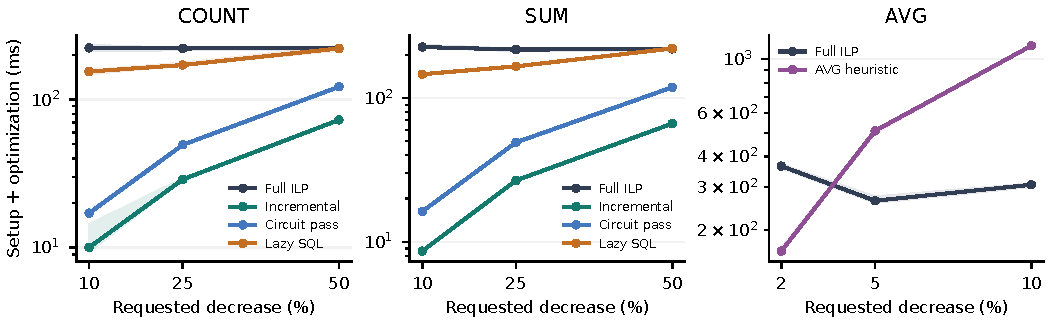
\includegraphics[width=\textwidth]{figures/evaluation_runtime.pdf}
\caption{TPC-H-derived pilot at SF 0.03. Points show median setup-plus-
optimization time over three repetitions; shaded ranges show the observed
minimum and maximum. The SQL method includes derivation-table
materialization. The circuit method is the specialized multilinear pass.
COUNT/SUM and AVG use different decrease ranges.}
\label{fig:pilot-runtime}
\Description{Three line plots compare median setup and optimization times at scale factor 0.03 as the requested decrease grows. Incremental coverage is fastest for COUNT and SUM. The AVG heuristic becomes slower than the full ILP at larger decreases. Shaded bands show the minimum and maximum of three timing repetitions.}
\end{figure*}

\subsection{Results and Interpretation}

\paragraph{Witness quality and correctness.}
All 180 returned sets passed both validation checks, all 54 ILP solves
reported optimality, and no run timed out. The exact-greedy variants agreed
on every selected tuple at each of the 12 COUNT/SUM cases. Their final
sizes matched the proven optimum in every case; AVG greedy also matched
it in all six AVG cases (Table~\ref{tab:pilot-sizes}). This is an observation
about the selected workload. For comparison, a four-derivation COUNT
control with supports $\{a,x\},\{a,y\},\{b,x\},\{c,y\}$ and full-loss
target has optimum $\{x,y\}$, whereas greedy with tuple order
$a,b,c,x,y$ selects $a,b,c$. Thus exact marginal computation does not make
greedy an exact optimization method in general.

\paragraph{Execution costs.}
At SF 0.03 and a 50\% COUNT decrease, median method time is 72.9\,ms for
incremental greedy, 121.9\,ms for the circuit pass, 221.5\,ms for lazy
SQL, and 222.0\,ms for ILP. All return size 311. Incremental greedy is
about $3.0\times$ faster than ILP in this cell. Its gains change only when
incident derivations die, whereas the circuit pass scans the surviving
contributions at every iteration. Lazy SQL reduces repeated gain
computation but also pays for its materialized table and SQL calls.
Figure~\ref{fig:pilot-runtime} shows the measured tradeoff across thresholds.

AVG illustrates a different cost profile. At SF 0.03 and a 10\% average
decrease, both methods return size 121, but the heuristic takes a median
1.132\,s versus 0.307\,s for ILP, about $3.7\times$ longer. The heuristic
repeatedly computes signed rational gains, while these small ILPs solve
quickly. A heuristic label therefore does not imply a runtime advantage.

\paragraph{Evaluation scope.}
The pilot validates three exact coverage implementations and a constructive
AVG search on one self-join-free join shape at two small scales. The timing
ranges characterize repeated execution of these inputs, rather than
variation across datasets. Larger databases, additional join shapes,
self-joins, extrema survivor enumeration, and peak memory remain necessary
dimensions of a broader scalability study. These distinctions keep
representation-level speedups separate from end-to-end workload claims.

\section{Related Work}
\label{sec:related}

\paragraph{Aggregated deletion propagation.}
Hu et al.~\cite{hu2021adp} study minimum source deletions to remove a prescribed
number of query outputs. In the shared
setting of full self-join-free queries over duplicate-free relations,
each full output corresponds to one derivation, so their ADP objective
is exactly our \agg{COUNT} objective. Their Theorem~6.2 gives
$O(\log k)$ and relation-count approximations, using partial set cover.
Bag projection here counts derivation copies;
set projection coalesces them and can change marginal behavior, as the
example in Section~\ref{sec:problem} shows. Weighted values, designated deletability, and aggregate validity conditions
require comparison under their actual semantics.

% Balance the final page with the class-provided balance package.
\balance
\paragraph{Generalized deletion propagation and resilience.}
Makhija and Gatterbauer~\cite{makhija2025ilp} unify deletion and preservation
requirements with source and view objectives. Their framework handles
self-joins and bags and gives ILP formulations with strong relaxation
properties in known tractable cases. Our survivor constraints and tuple-to-
derivation linking belong in this established methodological context.
The aggregate-specific inequalities in Section~\ref{sec:ilp} make our
threshold semantics explicit; we do not assert that this encoding is
outside their framework or has the same relaxation properties.

At $\theta=Q(D)>0$, \agg{COUNT} requires destroying all derivations,
which is query resilience with the same permitted deletions. Freire
et al.~\cite{freire2015resilience} study resilience as minimum deletions
making a Boolean conjunctive query false and characterize self-join-free
query classes. Our reduction uses a self-join and immutability; it neither
replaces that classification nor extends it to all aggregate queries.

\paragraph{Provenance and aggregate semantics.}
Semiring provenance represents the derivational dependence of positive
queries~\cite{green2007provenance}; aggregate provenance develops the
corresponding treatment of aggregate values~\cite{amsterdamer2011aggregate}.
We use fixed derivation values and deletable supports to reason about
interventions on that dependence. Our Boolean circuit contract is a
specific operational requirement for exact marginal computation, rather
than a claim that every provenance representation supplies the same oracle.
The multilinearity qualification is essential when tuple identifiers recur.

\paragraph{Submodular cover and bounded-rank hitting set.}
The logarithmic argument specializes the standard greedy analysis for
submodular covering~\cite{wolsey1982greedy}. The disjoint-support argument
is the elementary packing bound for bounded-rank hitting set. Our extrema
analysis uses these ingredients after selecting a survivor, so that an
otherwise feasible critical cover does not empty the aggregate input.
This interaction between threshold obligations and preservation matters
when applying deletion-propagation algorithms to aggregates that exclude
empty inputs.

\section{Discussion and Conclusion}
\label{sec:conclusion}

Minimum instability witnesses measure the permitted source deletions
needed to cross an aggregate threshold. Bag COUNT and nonnegative SUM
yield weighted coverage. Extrema yield critical-support hitting with a
surviving-derivation obligation, permitting a complete feasibility test and
a combined $\min\{r,1+\ln m\}$ approximation. AVG instead gives a signed
linear threshold over survivors. Fixed-query hardness coexists with exact
algorithms for singleton-support coverage and independent numeric rows.
Exact execution requires a specified representation: explicit-support
updates, query oracles, and circuit derivatives have different costs and
conditions of applicability.

\paragraph{Remaining theoretical questions.}
Our reduction does not classify all query shapes or establish matching
inapproximability. Safe-support enumeration can be expensive, motivating
compact survivor selection. Duplicate elimination, nulls, grouping, signed
SUM, and non-unit costs require separate analyses. AVG's failure of
numerical-benefit submodularity leaves open both richer tractable subclasses
and other approximation approaches.

\paragraph{Empirical questions.}
No dataset or runtime results are claimed here. An implementation study
should compare the exact ILP, incremental-support greedy, residual-query
greedy, and certified circuit greedy under identical semantics. It should
measure construction and optimization time, peak memory, oracle calls,
feasibility, and witness size. Optimality ratios require proven optima;
solver timeouts instead call for certified objective bounds. Varying join
multiplicity, self-joins, deletion policy, numerical precision, and distinct
safe supports would isolate the costs identified by the analysis and test
whether compact provenance offsets survivor enumeration.


\begingroup
% Keep individual reference paragraphs together across columns.
\interlinepenalty=10000
\bibliographystyle{ACM-Reference-Format}
\bibliography{references}
\endgroup

\end{document}
